\documentclass[../main.tex]{subfiles}

\newcolumntype{C}[1]{>{\centering\arraybackslash}m{#1}}

\begin{document}
\chapter{Rezultaty}

Metody przedstawione w poprzednich rozdziałach zostały zaimplementowane dla jednolitych świateł o prostokątnym kształcie. W tabelach \ref{tab:results:metal}, \ref{tab:results:conductor} przedstawione zostały rezultaty dla materiałów o stałych właściwościach przy zmiennej chropowatości powierzchni. Metoda referencyjna generuje 1280 próbek w celu wyznaczenia wartości całki (100 iteracji po 128 próbek każda).

W tabeli \ref{tab:performance} zostały przedstawione średnie czasy generowania jednej ramki obrazu. Platforma testowa posiada składa się z procesora i5-8600K 3.60GHz, 16GB pamięci RAM i karty graficznej NVIDIA GeForce GTX1080.

Z tych rezultatów możemy wyciągnąć wniosek, że metoda chmury świateł punktowych nie skaluje się dobrze oraz nie spełnia swojej funkcji przy niskich wartościach chropowatości, dla odpowiednio niskich wartości wyraźnie widać strukturę światła powierzchniowego (rys. \ref{fig:results:pointManyLowAlpha}).

\begin{figure}[h]
    \centering
    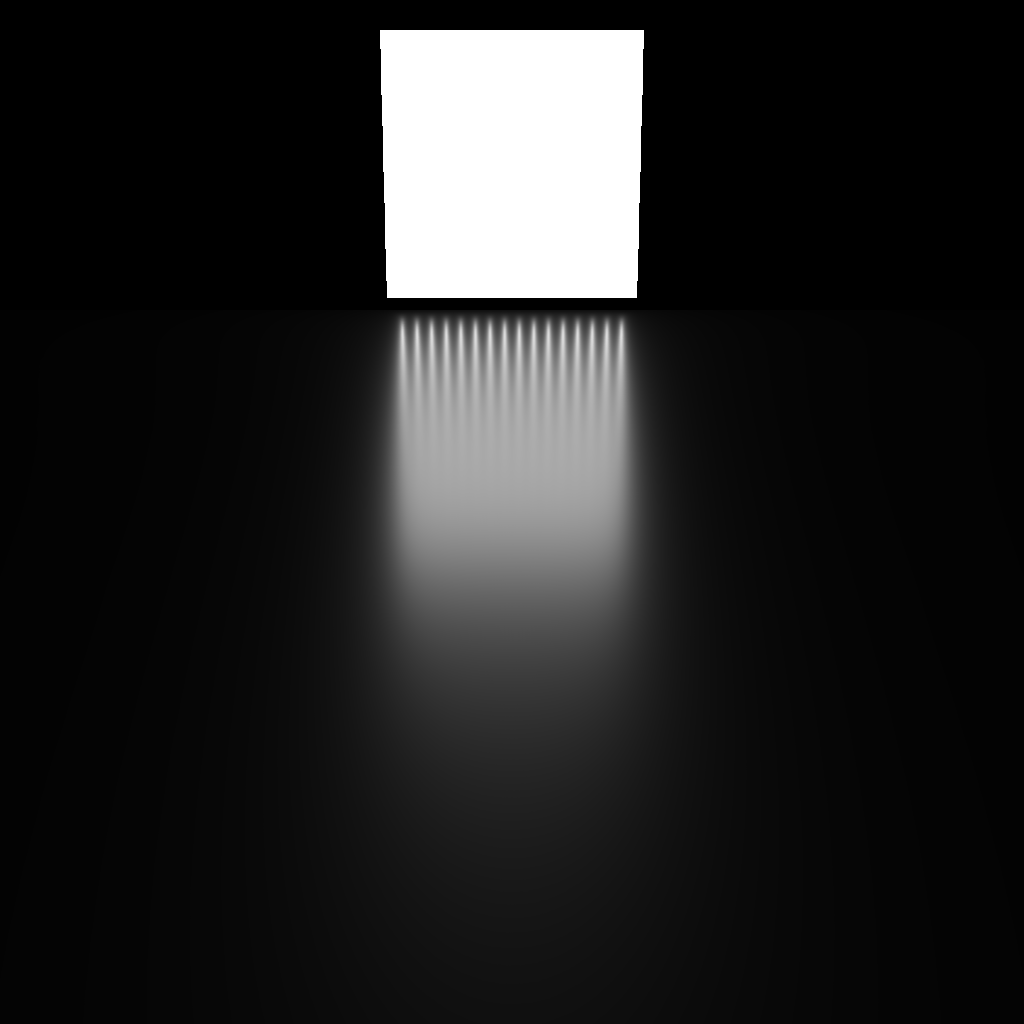
\includegraphics[width=0.4\linewidth]{results/misc/point-16x16-low-alpha}
    \caption{Klaster świateł punktowych 16 na 16 przy niskiej chropowatości. Opracowanie własne.}
    \label{fig:results:pointManyLowAlpha}
\end{figure}

Metoda liniowo przekształconych kosinusów wygenerowała satysfakcjonujące rezultaty dla większości 

\begin{table}[h]
    \centering
    \begin{tabular}{C{0.5cm}C{4cm}C{4cm}C{4cm}}
        $\alpha$ & Monte-Carlo & Światła punktowe (8x8) & LTC \\
        $0.2$ 
            & \includegraphics[width=4cm]{results/metal/{gt-flux-10-roughness-0.2}.png}
            & \includegraphics[width=4cm]{results/metal/{ltc-flux-10-roughness-0.2}.png}
            & \includegraphics[width=4cm]{results/metal/{point-flux-10-roughness-0.2}.png} \\
        $0.4$ 
            & \includegraphics[width=4cm]{results/metal/{gt-flux-10-roughness-0.4}.png}
            & \includegraphics[width=4cm]{results/metal/{ltc-flux-10-roughness-0.4}.png}
            & \includegraphics[width=4cm]{results/metal/{point-flux-10-roughness-0.4}.png} \\
        $0.6$
            & \includegraphics[width=4cm]{results/metal/{gt-flux-10-roughness-0.6}.png}
            & \includegraphics[width=4cm]{results/metal/{ltc-flux-10-roughness-0.6}.png}
            & \includegraphics[width=4cm]{results/metal/{point-flux-10-roughness-0.6}.png} \\
        $0.8$ 
            & \includegraphics[width=4cm]{results/metal/{gt-flux-10-roughness-0.8}.png}
            & \includegraphics[width=4cm]{results/metal/{ltc-flux-10-roughness-0.8}.png}
            & \includegraphics[width=4cm]{results/metal/{point-flux-10-roughness-0.8}.png} \\
        $1.0$ 
            & \includegraphics[width=4cm]{results/metal/{gt-flux-10-roughness-1}.png}
            & \includegraphics[width=4cm]{results/metal/{ltc-flux-10-roughness-1}.png}
            & \includegraphics[width=4cm]{results/metal/{point-flux-10-roughness-1}.png}
    \end{tabular}
    \caption{Jednolita metalowa powierzchnia o różnym współczynniku chropowatości $\alpha$. Opracowanie własne.}
    \label{tab:results:metal}
\end{table}

\begin{table}[h]
    \centering
    \begin{tabular}{C{0.5cm}C{4cm}C{4cm}C{4cm}}
        $\alpha$ & Monte-Carlo & Światła punktowe (8x8) & LTC \\
        $0.2$ 
        & \includegraphics[width=4cm]{results/conductor/{gt-flux-10-roughness-0.2}.png}
        & \includegraphics[width=4cm]{results/conductor/{ltc-flux-10-roughness-0.2}.png}
        & \includegraphics[width=4cm]{results/conductor/{point-flux-10-roughness-0.2}.png} \\
        $0.4$ 
        & \includegraphics[width=4cm]{results/conductor/{gt-flux-10-roughness-0.4}.png}
        & \includegraphics[width=4cm]{results/conductor/{ltc-flux-10-roughness-0.4}.png}
        & \includegraphics[width=4cm]{results/conductor/{point-flux-10-roughness-0.4}.png} \\
        $0.6$
        & \includegraphics[width=4cm]{results/conductor/{gt-flux-10-roughness-0.6}.png}
        & \includegraphics[width=4cm]{results/conductor/{ltc-flux-10-roughness-0.6}.png}
        & \includegraphics[width=4cm]{results/conductor/{point-flux-10-roughness-0.6}.png} \\
        $0.8$ 
        & \includegraphics[width=4cm]{results/conductor/{gt-flux-10-roughness-0.8}.png}
        & \includegraphics[width=4cm]{results/conductor/{ltc-flux-10-roughness-0.8}.png}
        & \includegraphics[width=4cm]{results/conductor/{point-flux-10-roughness-0.8}.png} \\
        $1.0$ 
        & \includegraphics[width=4cm]{results/conductor/{gt-flux-10-roughness-1}.png}
        & \includegraphics[width=4cm]{results/conductor/{ltc-flux-10-roughness-1}.png}
        & \includegraphics[width=4cm]{results/conductor/{point-flux-10-roughness-1}.png}
    \end{tabular}
    \caption{Izolator o różnym współczynniku chropowatości $\alpha$. Opracowanie własne.}
    \label{tab:results:conductor}
\end{table}

\end{document}
